% Options for packages loaded elsewhere
\PassOptionsToPackage{unicode}{hyperref}
\PassOptionsToPackage{hyphens}{url}
%
\documentclass[
  ignorenonframetext,
]{beamer}
\usepackage{pgfpages}
\setbeamertemplate{caption}[numbered]
\setbeamertemplate{caption label separator}{: }
\setbeamercolor{caption name}{fg=normal text.fg}
\beamertemplatenavigationsymbolsempty
% Prevent slide breaks in the middle of a paragraph
\widowpenalties 1 10000
\raggedbottom
\setbeamertemplate{part page}{
  \centering
  \begin{beamercolorbox}[sep=16pt,center]{part title}
    \usebeamerfont{part title}\insertpart\par
  \end{beamercolorbox}
}
\setbeamertemplate{section page}{
  \centering
  \begin{beamercolorbox}[sep=12pt,center]{part title}
    \usebeamerfont{section title}\insertsection\par
  \end{beamercolorbox}
}
\setbeamertemplate{subsection page}{
  \centering
  \begin{beamercolorbox}[sep=8pt,center]{part title}
    \usebeamerfont{subsection title}\insertsubsection\par
  \end{beamercolorbox}
}
\AtBeginPart{
  \frame{\partpage}
}
\AtBeginSection{
  \ifbibliography
  \else
    \frame{\sectionpage}
  \fi
}
\AtBeginSubsection{
  \frame{\subsectionpage}
}
\usepackage{amsmath,amssymb}
\usepackage{iftex}
\ifPDFTeX
  \usepackage[T1]{fontenc}
  \usepackage[utf8]{inputenc}
  \usepackage{textcomp} % provide euro and other symbols
\else % if luatex or xetex
  \usepackage{unicode-math} % this also loads fontspec
  \defaultfontfeatures{Scale=MatchLowercase}
  \defaultfontfeatures[\rmfamily]{Ligatures=TeX,Scale=1}
\fi
\usepackage{lmodern}
\usecolortheme{spruce}
\ifPDFTeX\else
  % xetex/luatex font selection
\fi
% Use upquote if available, for straight quotes in verbatim environments
\IfFileExists{upquote.sty}{\usepackage{upquote}}{}
\IfFileExists{microtype.sty}{% use microtype if available
  \usepackage[]{microtype}
  \UseMicrotypeSet[protrusion]{basicmath} % disable protrusion for tt fonts
}{}
\makeatletter
\@ifundefined{KOMAClassName}{% if non-KOMA class
  \IfFileExists{parskip.sty}{%
    \usepackage{parskip}
  }{% else
    \setlength{\parindent}{0pt}
    \setlength{\parskip}{6pt plus 2pt minus 1pt}}
}{% if KOMA class
  \KOMAoptions{parskip=half}}
\makeatother
\usepackage{xcolor}
\newif\ifbibliography
\usepackage{graphicx}
\makeatletter
\def\maxwidth{\ifdim\Gin@nat@width>\linewidth\linewidth\else\Gin@nat@width\fi}
\def\maxheight{\ifdim\Gin@nat@height>\textheight\textheight\else\Gin@nat@height\fi}
\makeatother
% Scale images if necessary, so that they will not overflow the page
% margins by default, and it is still possible to overwrite the defaults
% using explicit options in \includegraphics[width, height, ...]{}
\setkeys{Gin}{width=\maxwidth,height=\maxheight,keepaspectratio}
% Set default figure placement to htbp
\makeatletter
\def\fps@figure{htbp}
\makeatother
\setlength{\emergencystretch}{3em} % prevent overfull lines
\providecommand{\tightlist}{%
  \setlength{\itemsep}{0pt}\setlength{\parskip}{0pt}}
\setcounter{secnumdepth}{-\maxdimen} % remove section numbering
\setbeamercovered{transparent=30}
\ifLuaTeX
  \usepackage{selnolig}  % disable illegal ligatures
\fi
\IfFileExists{bookmark.sty}{\usepackage{bookmark}}{\usepackage{hyperref}}
\IfFileExists{xurl.sty}{\usepackage{xurl}}{} % add URL line breaks if available
\urlstyle{same}
\hypersetup{
  pdftitle={A dive into the wastewater-based epidemiology of SARS-CoV in Switzerland},
  pdfauthor={Julien Riou},
  hidelinks,
  pdfcreator={LaTeX via pandoc}}

\title{A dive into the wastewater-based epidemiology of SARS-CoV in
Switzerland}
\subtitle{Colloque scientifique mensuel ESD}
\author{Julien Riou}
\date{7 November 2023}

\begin{document}
\frame{\titlepage}

\begin{frame}{Disease surveillance}
\protect\hypertarget{disease-surveillance}{}
Definition \emph{(Langmuir, 1963)}:

\bigskip

\begin{quote}
Surveillance, when applied to a disease, means the \alert{continued watchfulness} over the distribution and trends of incidence through the systematic \alert{collection}, \alert{consolidation} and \alert{evaluation} of morbidity and mortality reports and other relevant data.
\end{quote}
\end{frame}

\begin{frame}{Objectives of disease surveillance \emph{(Declich, 1994)}}
\protect\hypertarget{objectives-of-disease-surveillance-declich-1994}{}
To describe the \alert{ongoing patterns} of disease:

\begin{itemize}
\tightlist
\item
  identify trends and acute changes \pause\medskip
\end{itemize}

To link with \alert{public health action}:

\begin{itemize}
\item
  disease investigation and control
\item
  health services planning
\item
  evaluation of measures \pause\medskip
\end{itemize}

To study the \alert{natural history} and \alert{epidemiology} of
diseases:

\begin{itemize}
\tightlist
\item
  not limited to those diseases for which effective control measures are
  available
\end{itemize}
\end{frame}

\begin{frame}{Historical origins of disease surveillance}
\protect\hypertarget{historical-origins-of-disease-surveillance}{}
\begin{figure}
\centering
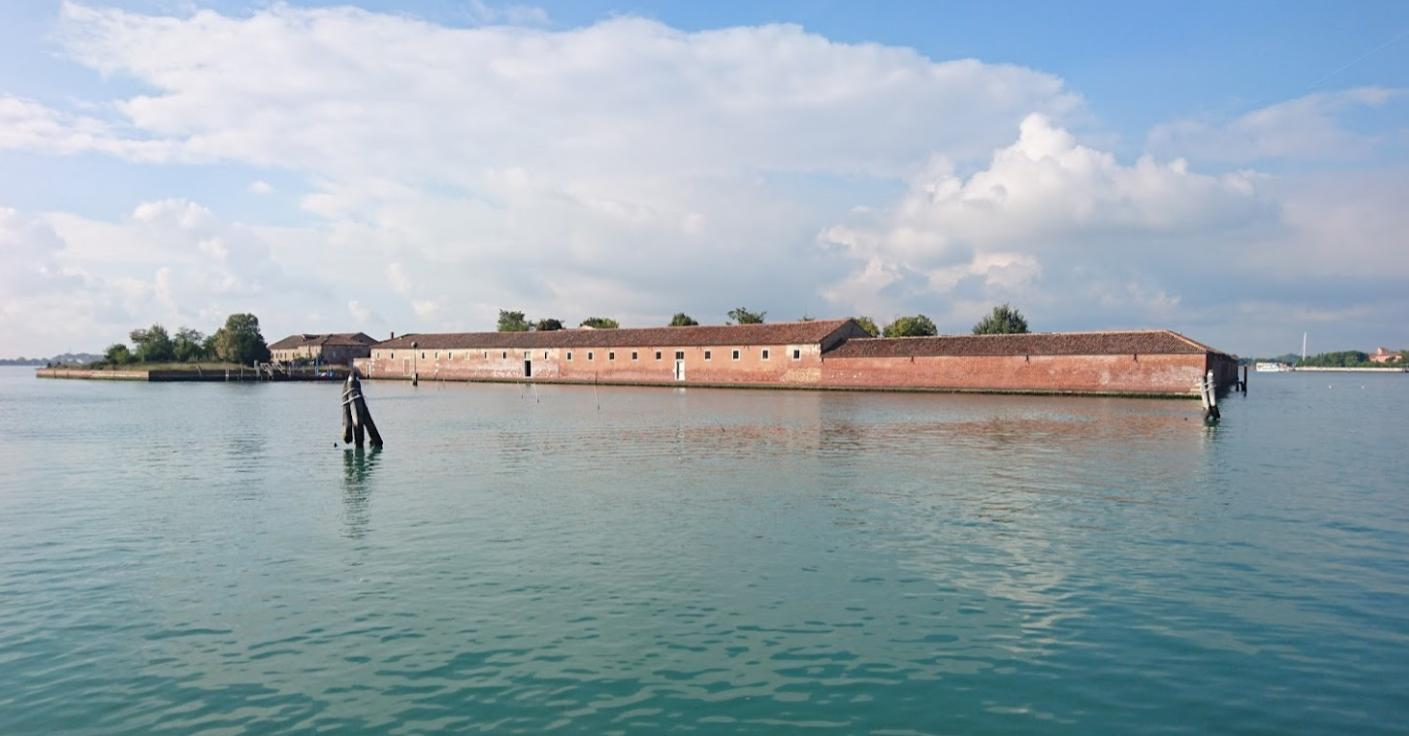
\includegraphics[width=\linewidth]{figures/isolation_hospital_lazzaretto_vecchio_wikicommons.jpg}
\caption{The quarantine hospital on Lazzaretto Vecchio island was at the center of Venice's vast \alert{public health response} to the Black Death in the 14th century \textit{(Wikimedia commons)}.}
\end{figure}
\end{frame}

\begin{frame}{Historical origins of disease surveillance}
\protect\hypertarget{historical-origins-of-disease-surveillance-1}{}
\begin{figure}
\centering
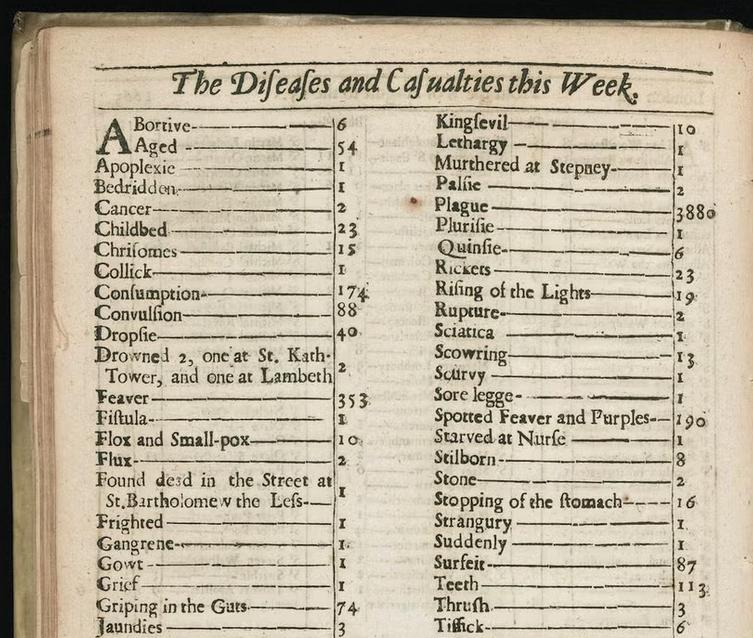
\includegraphics[width=.7\linewidth]{figures/london_bill_of_mortality_1664.jpg}
\caption{In 17th-century London, in response to recurrences of bubonic plague, authorities instituted the weekly publication of a \alert{Bill of Mortality} detailing the number of burials with cause of death \textit{(Wellcome Library)}.}
\end{figure}
\end{frame}

\begin{frame}{Historical origins of disease surveillance}
\protect\hypertarget{historical-origins-of-disease-surveillance-2}{}
\begin{figure}
\centering
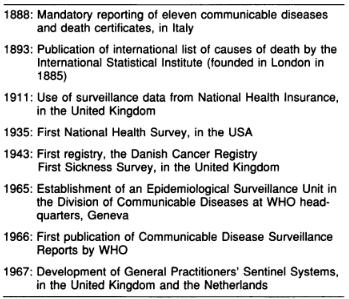
\includegraphics[width=.5\linewidth]{figures/declich_developments_20th_Century.jpg}
\caption{Developments of disease surveillance since the end of the 19th century \textit{(Declich, 1994)}.}
\end{figure}
\end{frame}

\begin{frame}{Infectious disease surveillance today}
\protect\hypertarget{infectious-disease-surveillance-today}{}
Passive surveillance:

\begin{itemize}
\item
  \alert{mandatory notification} of cases by doctors and labs
\item
  administrative data (encoded hospital billing data)
\item
  vital statistics \pause\bigskip
\end{itemize}

Active surveillance:

\begin{itemize}
\item
  outbreak investigation
\item
  sentinel systems
\item
  population-based surveys
\item
  \alert{wastewater-based epidemiology}
\end{itemize}
\end{frame}

\begin{frame}{Background}
\protect\hypertarget{background}{}
Wastewater-based epidemiology (WBE):

\begin{itemize}
\item
  first proposed by Daughton (2001) for monitoring \alert{illicit drugs}
\item
  extension to pharmaceuticals, tobacco, alcohol, pesticides, heavy
  metals\ldots{} (Choi, 2018)
\item
  extension to \alert{infectious diseases} (Mao, 2020)
\end{itemize}
\end{frame}

\begin{frame}{Background}
\protect\hypertarget{background-1}{}
WBE for infectious disease surveillance:

\begin{itemize}
\item
  \alert{early warning signals} (identify circulating
  pathogens/variants)
\item
  \alert{spatio-temporal trends?}
\end{itemize}

\begin{figure}
\centering

\includegraphics[width=.5\linewidth]{figures/wastewater-surveillance-illustration-cdc}
\caption{WBE for infectious disease surveillance \textit{(CDC)}.}
\end{figure}
\end{frame}

\begin{frame}{Background}
\protect\hypertarget{background-2}{}
Data-generating mechanism:

\begin{itemize}
\item
  SARS-CoV-2 incidence
\item
  \alert{Fecal shedding profile} (1-2 weeks, up to 7 months)
\item
  Circulation in wastewater pipes, sample collection
\item
  Quantification with RT-PCR
\end{itemize}

\begin{figure}
\centering
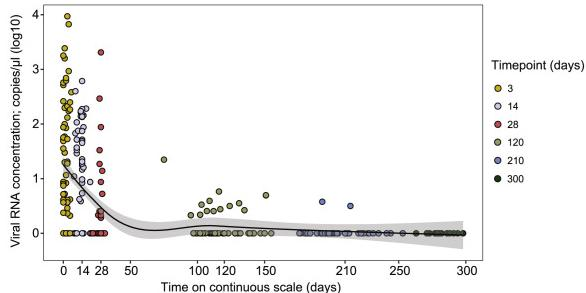
\includegraphics[width=.5\linewidth]{figures/shedding}
\caption{Fecal viral RNA concentration in stool samples over time \textit{(Natarajan et al., 2022)}.}
\end{figure}
\end{frame}

\begin{frame}{Data}
\protect\hypertarget{data}{}
Wastewater surveillance of SARS-CoV-2 in Switzerland:

\begin{itemize}
\item
  started 7 February 2022
\item
  maximal \alert{118 wastewater plants} (ARA for
  \emph{Abwasserreinigungsanlagen})
\item
  fluctuations in the number of ARAs, down to 14 after July 2023
\item
  various sampling frequencies (3 to 6 times per week)
\item
  samples sent to \alert{9 different laboratories} (1 lab after July
  2023)
\item
  22367 total measurements as of 18 September 2023
\end{itemize}
\end{frame}

\begin{frame}{Data}
\protect\hypertarget{data-1}{}
Raw data consists of \alert{concentrations} in gene copies per liter
{[}gc/L{]}

\begin{itemize}
\item
  account for \alert{wastewater flow} {[}m3/day{]} (rain,
  activity\ldots)
\item
  account for \alert{population} covered by the ARA
\item
  formula for \alert{viral load per population} {[}gc/day/100,000
  population{]}
\end{itemize}

\[
VL = \frac{\text{concentration} \times \text{flow} \times 1,000}{\text{population} / 100,000}
\]
\end{frame}

\begin{frame}{Data}
\protect\hypertarget{data-2}{}
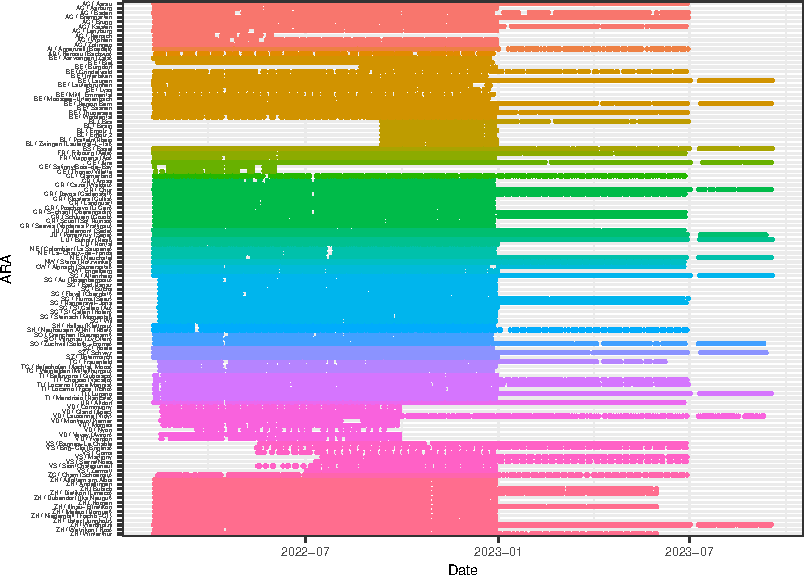
\includegraphics{2023-11-07_pres_files/figure-beamer/data_mis1-1.pdf}
\end{frame}

\begin{frame}{Data}
\protect\hypertarget{data-3}{}
\begin{figure}
\centering
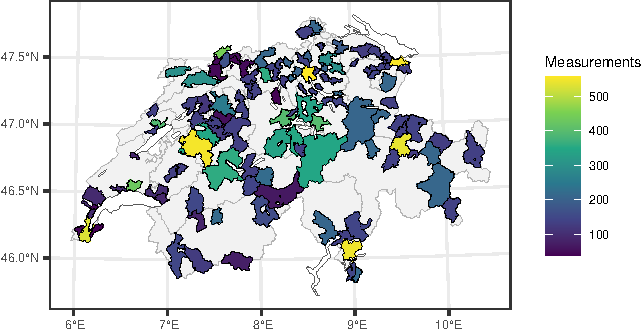
\includegraphics{2023-11-07_pres_files/figure-beamer/data_mis2-1.pdf}
\caption{Number of viral load measurements by ARA.}
\end{figure}
\end{frame}

\begin{frame}{Data}
\protect\hypertarget{data-4}{}
Large \alert{heterogeneity} across time and space:

\begin{figure}
\centering
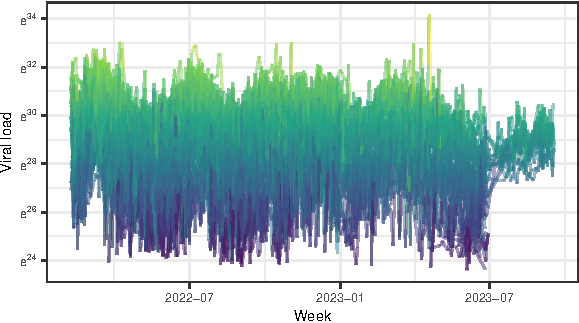
\includegraphics{2023-11-07_pres_files/figure-beamer/data_vl1-1.pdf}
\caption{Daily SARS-CoV-2 viral load in wastewater by ARA (removing
values below the LOD or LOQ).}
\end{figure}
\end{frame}

\begin{frame}{Data}
\protect\hypertarget{data-5}{}
Difficulties of \alert{interpretation}:

\begin{figure}
\centering
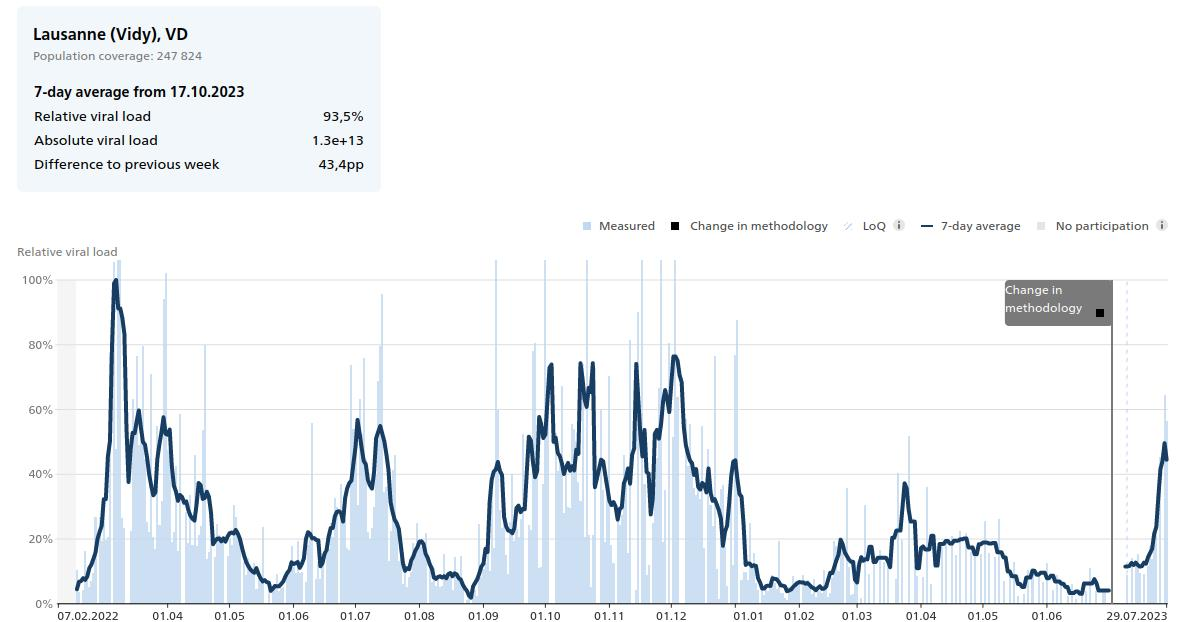
\includegraphics[width=.9\linewidth]{figures/lausanne}
\caption{Viral load in wastewater as of 31 October 2023, Lausanne VD (Vidy) \textit{(FOPH dashboard, covid19.admin.ch)}.}
\end{figure}
\end{frame}

\begin{frame}{Objectives}
\protect\hypertarget{objectives}{}
\begin{enumerate}
\tightlist
\item
  Disentangle the \alert{various sources of heterogeneity}
\end{enumerate}

\begin{itemize}
\tightlist
\item
  laboratory, quantification method, systematic temporal or spatial
  effects, remaining noise\ldots{} \pause\bigskip
\end{itemize}

\begin{enumerate}
\setcounter{enumi}{1}
\tightlist
\item
  Extract a clean, ``noise-free'\,' \alert{temporal signal}
\end{enumerate}

\begin{itemize}
\tightlist
\item
  at the national and/or regional level \pause\bigskip
\end{itemize}

\begin{enumerate}
\setcounter{enumi}{2}
\tightlist
\item
  Assess the \alert{agreement} with other types of surveillance
\end{enumerate}

\begin{itemize}
\tightlist
\item
  confirmed cases, hospitalizations, Sentinella, CH-SUR, pooled
  tests\ldots{} \pause\bigskip
\end{itemize}
\end{frame}

\begin{frame}{Objectives}
\protect\hypertarget{objectives-1}{}
\begin{enumerate}
\setcounter{enumi}{3}
\tightlist
\item
  Forecasting/nowcasting
\end{enumerate}

\begin{itemize}
\tightlist
\item
  historical data, LFO validation \pause\bigskip
\end{itemize}

\begin{enumerate}
\setcounter{enumi}{4}
\tightlist
\item
  Future surveillance strategies
\end{enumerate}

\begin{itemize}
\tightlist
\item
  site selection, sampling frequency, rotation
\end{itemize}
\end{frame}

\begin{frame}{Methods}
\protect\hypertarget{methods}{}
\alert{Space-time} model based on gamma regression, accounting for:

\begin{itemize}
\item
  limits of detection (LOD) and of quantification (LOQ)\pause
\item
  systematic temporal effects (public holidays, weekends) \pause
\item
  national \alert{time trend} (RW2)
\item
  \alert{systematic shift} for each ARA (IID)
\item
  deviations from national trend for each ARA (RW1) \pause
\item
  effect of \alert{laboratory} and quantification method
\end{itemize}
\end{frame}

\begin{frame}{Results}
\protect\hypertarget{results}{}
Posterior predictive check (\alert{model fit}) is quite good.

\begin{figure}
\centering
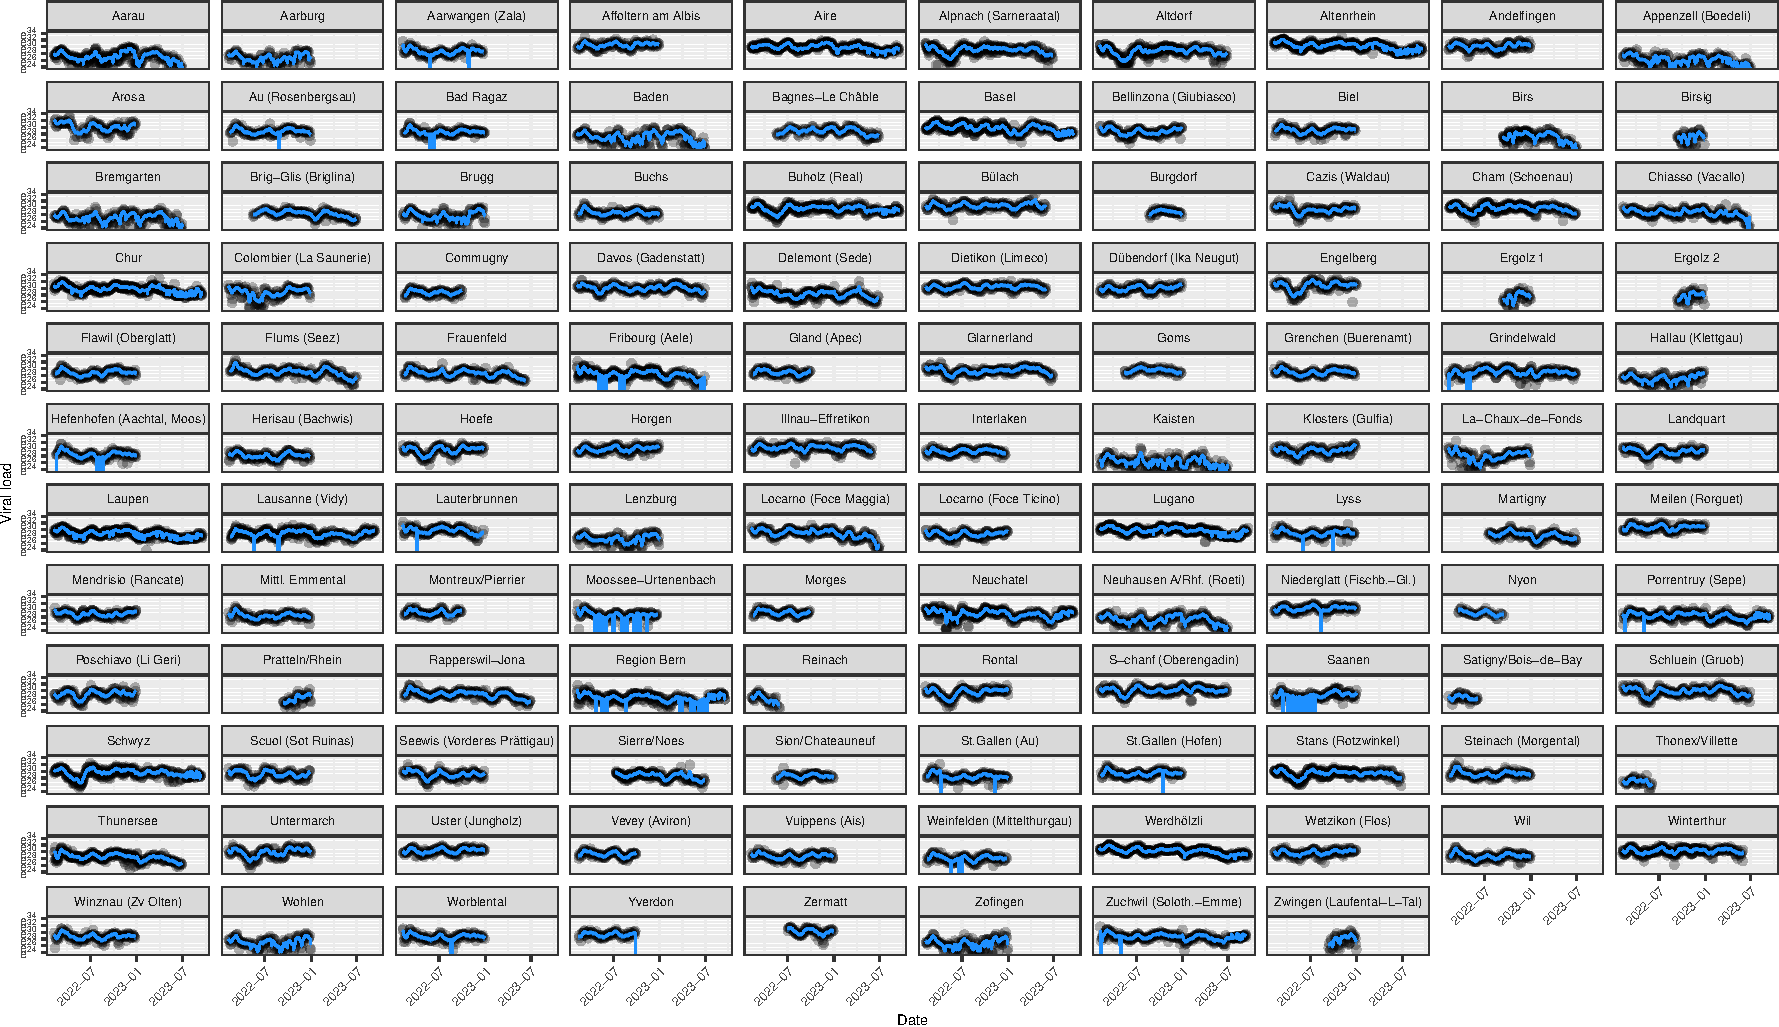
\includegraphics{2023-11-07_pres_files/figure-beamer/res_fit1-1.pdf}
\caption{Model fit.}
\end{figure}
\end{frame}

\begin{frame}{Results}
\protect\hypertarget{results-1}{}
Posterior predictive check (\alert{model fit}) is generally quite good.

\begin{figure}
\centering
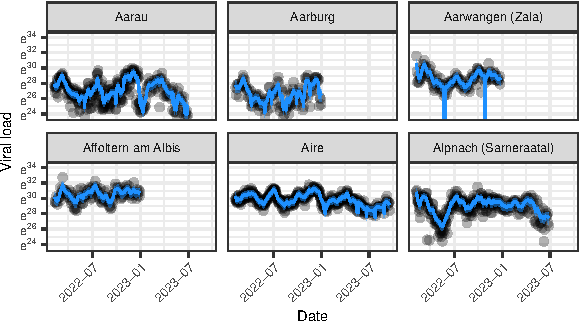
\includegraphics{2023-11-07_pres_files/figure-beamer/res_fit2-1.pdf}
\caption{Model fit.}
\end{figure}
\end{frame}

\begin{frame}{Results}
\protect\hypertarget{results-2}{}
Effect of \alert{laboratory} and method (reference is EAWAG\_0):

\begin{itemize}
\tightlist
\item
  \(\exp(\beta)\) can be interpreted as a \alert{relative viral load},
  e.g., the viral load is \emph{on average} 1.39 times higher (0.88 to
  2.18) in KLZH than EAWAG\_0
\end{itemize}

\begin{figure}
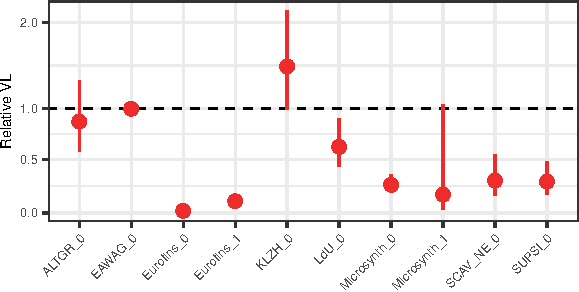
\includegraphics[width=0.7\linewidth]{2023-11-07_pres_files/figure-beamer/res1-1} \caption{Estimated effect of laboratory (laboratory name) and method change (marked by 0 and 1).}\label{fig:res1}
\end{figure}
\end{frame}

\begin{frame}{Results}
\protect\hypertarget{results-3}{}
Effect of \alert{public holidays} and \alert{weekends}:

\begin{itemize}
\tightlist
\item
  no clear influence
\end{itemize}

\begin{figure}
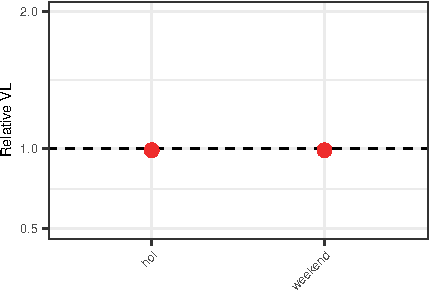
\includegraphics[width=0.5\linewidth]{2023-11-07_pres_files/figure-beamer/res2-1} \caption{Estimated effect of holidays and weekends.}\label{fig:res2}
\end{figure}
\end{frame}

\begin{frame}{Results}
\protect\hypertarget{results-4}{}
Effect of \alert{specific ARAs}:

\begin{itemize}
\item
  some ARAs have consistently higher or lower viral loads
\item
  may be issues with \alert{population} covered (tourism\ldots)
\end{itemize}

\begin{figure}
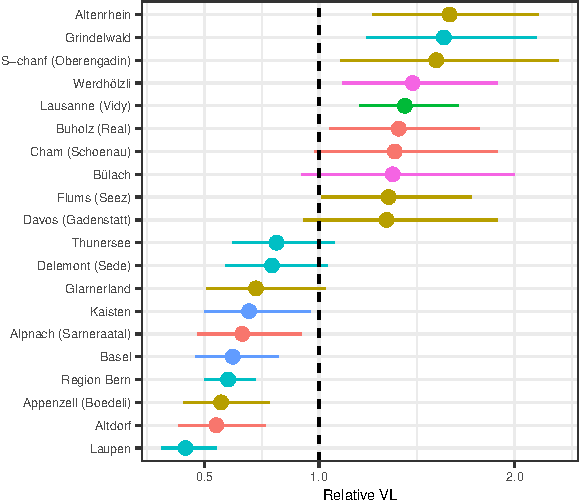
\includegraphics[width=0.5\linewidth]{2023-11-07_pres_files/figure-beamer/res3-1} \caption{Estimated ARA-specific effects.}\label{fig:res3}
\end{figure}
\end{frame}

\begin{frame}{Results}
\protect\hypertarget{results-5}{}
Effect of \alert{specific ARAs}:

\begin{itemize}
\item
  some ARAs have consistently higher or lower viral loads
\item
  may be issues with \alert{population} covered (tourism\ldots)
\end{itemize}

\begin{figure}
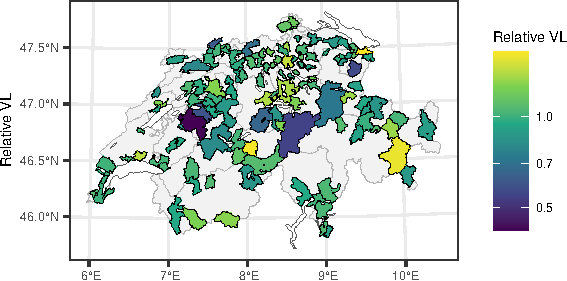
\includegraphics[width=0.8\linewidth]{2023-11-07_pres_files/figure-beamer/res4-1} \caption{Estimated ARA-specific effects.}\label{fig:res4}
\end{figure}
\end{frame}

\begin{frame}{Results}
\protect\hypertarget{results-6}{}
Average temporal trend at the \alert{national} level:

\begin{itemize}
\tightlist
\item
  accounts for all aspects described before
\end{itemize}

\begin{figure}
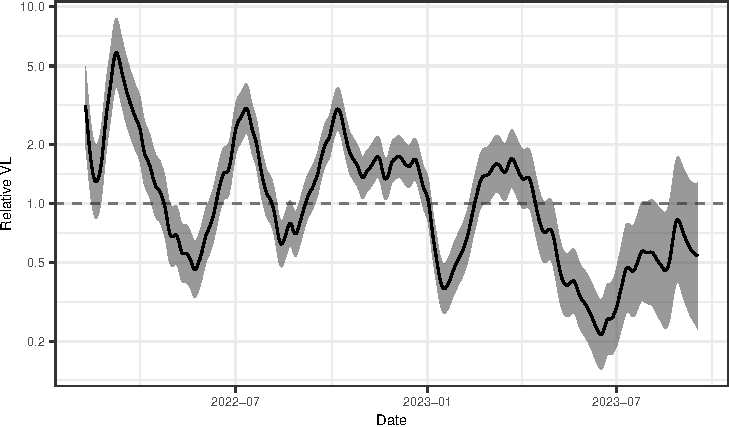
\includegraphics[width=0.8\linewidth]{2023-11-07_pres_files/figure-beamer/res5-1} \caption{Estimated average temporal trend at the national level.}\label{fig:res5}
\end{figure}
\end{frame}

\begin{frame}{Results}
\protect\hypertarget{results-7}{}
\alert{Residual deviations} from the average temporal trend:

\begin{itemize}
\tightlist
\item
  come on top of all aspects described before
\end{itemize}

\begin{figure}
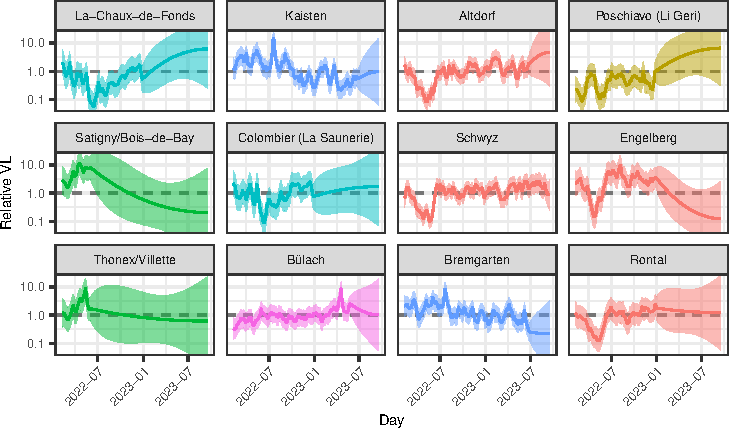
\includegraphics[width=0.8\linewidth]{2023-11-07_pres_files/figure-beamer/res7-1} \caption{Residual deviations from the average temporal trend (top 12 on absolute value).}\label{fig:res7}
\end{figure}
\end{frame}

\begin{frame}{Discussion}
\protect\hypertarget{discussion}{}
\begin{enumerate}
\tightlist
\item
  Disentangle the \alert{various sources of heterogeneity}
\end{enumerate}

\begin{itemize}
\item
  important heterogeneity across \alert{laboratories} and \alert{ARAs}
\item
  no clear effect of weekends and public holidays
\item
  possible issue with \alert{population} covered (tourism and/or
  mistake) \pause\bigskip
\end{itemize}

\begin{enumerate}
\setcounter{enumi}{1}
\tightlist
\item
  Extract a clean, ``noise-free'\,' \alert{temporal signal}
\end{enumerate}

\begin{itemize}
\item
  national time trend
\item
  local trends to identify special situations (Neuchâtel-Jura / Berner
  Oberland)
\end{itemize}
\end{frame}

\begin{frame}{Discussion}
\protect\hypertarget{discussion-1}{}
Future work:

\begin{itemize}
\item
  Additional \alert{covariates}: socio-economic position (SEP),
  population density, urban/rural, working population, ethnicity\ldots{}
  \pause
\item
  Assess the \alert{agreement} with other types of surveillance (obj. 3;
  joint modelling of reported cases/hospitalizations and viral load)
  \pause
\item
  Move on to \alert{forecasting/nowcasting} (obj. 4) and
  \alert{surveillance strategies} (obj. 5) using the clean temporal
  signal (from obj. 2)
\end{itemize}
\end{frame}

\begin{frame}{Acknowledgements}
\protect\hypertarget{acknowledgements}{}
FOPH: Anna Fesser, Moritz Wagner, Katrin Schneider

ETHZ: James Munday, Tanja Stadler

EAWAG: Tim Julian, Christopher Ort
\end{frame}

\end{document}
